\documentclass[11pt,titlepage]{article}
\usepackage{ucs}
\usepackage[utf8x]{inputenc}
\usepackage[T1]{fontenc}
\usepackage[ngerman]{babel}
\usepackage{graphicx}
\usepackage{titlesec}
\usepackage{url}
\usepackage{lastpage}
\usepackage{listings}
\usepackage{color}
\usepackage{fancyhdr}
\usepackage{geometry}
\usepackage{wrapfig}
\usepackage{float}
\usepackage{subcaption}
\usepackage{hyperref}
\hypersetup{
    colorlinks=true,
    linkcolor=black,
    anchorcolor=black,
	citecolor=black,
	filecolor=black,
	menucolor=black,
	runcolor=black,
    urlcolor=blue,
	linktoc=all,
    pdftitle={Linux Networking},
    pdfauthor={Markus Gachnang und Martin Sprecher}
}
\usepackage{ragged2e}
\usepackage{framed}
\usepackage{quoting}
\usepackage{lscape}
\usepackage[table]{xcolor}
\usepackage{graphicx} 
\usepackage{pdfpages}
% remove current style and use fancyplain
\pagestyle{fancyplain}
\fancyhf{}
% remove rule/lines as well
\renewcommand{\headrulewidth}{0pt}
\renewcommand{\footrulewidth}{0pt}
% set papersize, magin and footersize
\geometry{a4paper,portrait,left={3cm},right={3cm},top={2cm},bottom={1cm},includefoot,foot={1cm}}
% set footer
\rfoot{Seite \thepage \hspace{1pt} von \pageref{LastPage}}
% Bibliographie
\usepackage{cite}
\def\BibTeX{{\rm B\kern-.05em{\sc i\kern-.025em b}\kern-.08em
    T\kern-.1667em\lower.7ex\hbox{E}\kern-.125emX}}
% define some colors
\definecolor{lightgray}{rgb}{.95,.95,.95}
\definecolor{shadecolor}{rgb}{.95,.95,.95}
\definecolor{darkgray}{rgb}{.4,.4,.4}
\definecolor{purple}{rgb}{0.65, 0.12, 0.82}
% set color and font of ''\url''
\renewcommand\UrlFont{\color{blue}\rmfamily\itshape}
% colorbox which can wrap lines
\newcommand\code[1]{\codehelp#1 \relax\relax}
\def\codehelp#1 #2\relax{\allowbreak\grayspace\codecolor{#1}\ifx\relax#2\else
 \codehelp#2\relax\fi}
\newcommand\codecolor[1]{\colorbox{lightgray}{\textcolor{black}{%
  \ttfamily\mystrut\smash{\detokenize{#1}}}}}
\def\mystrut{\rule[\dimexpr-\dp\strutbox+\fboxsep]{0pt}{%
 \dimexpr\normalbaselineskip-2\fboxsep}}
\def\grayspace{\hspace{0pt minus \fboxsep}}
% add ''\code'' to highligth single code lines
%\newcommand{\code}[1]{\wrapcolorbox[lightgray]{\ttfamily{#1}}}

% add ''\shadedquotation'' to highligth quoates
\newenvironment{shadedquotation}
 {\begin{shaded*}
  \quoting[leftmargin=0pt, vskip=0pt]
 }
 {\endquoting
 \end{shaded*}
}

% define ''JavaScript'' as a language for enviroment ''lstlisting''
\lstdefinelanguage{JavaScript}{
  keywords={typeof, new, true, false, catch, function, return, null, catch, switch, var, if, in, while, do, else, case, break},
  keywordstyle=\color{blue}\bfseries,
  ndkeywords={class, export, boolean, throw, implements, import, this},
  ndkeywordstyle=\color{darkgray}\bfseries,
  identifierstyle=\color{black},
  sensitive=false,
  comment=[l]{//},
  morecomment=[s]{/*}{*/},
  commentstyle=\color{purple}\ttfamily,
  stringstyle=\color{red}\ttfamily,
  morestring=[b]',
  morestring=[b]''
}

\lstset{
   language=JavaScript,
   backgroundcolor=\color{lightgray},
   extendedchars=true,
   basicstyle=\footnotesize\ttfamily,
   showstringspaces=false,
   showspaces=false,
   numbers=left,
   numberstyle=\footnotesize,
   numbersep=9pt,
   tabsize=2,
   breaklines=true,
   showtabs=false,
   captionpos=b
}
% set title
\title{Linux Networking}
\author{Markus Gachnang und Martin Sprecher}
\date{\today{}}
% set parindent to 0px to remove it (Einrücken von neuer Absatz)
\setlength\parindent{0pt}
% ---------------------------------------------------------------------------
% begin Document
\begin{document}
% set font
\sffamily
% print title
\maketitle
\newpage
% print index
\tableofcontents{}
\setcounter{page}{1}
\newpage
% linksbündig
\RaggedRight
% kein brechen von Wörtern
\tolerance=1
\emergencystretch=\maxdimen
\hyphenpenalty=10000
\hbadness=10000

\section{Ausgangslage}
\label{sec:Ausgangslage}


\section{Kochbuch}
\label{sec:Kochbuch}

\begin{shadedquotation}
  It is expected of you to hand in a step-by-step cookbook for the whole final setup. Explain important commands and reason your decisions. We should be able to fully retrace what you did to be able to assess your work. One cookbook is expected per group.
\end{shadedquotation}

\subsection{General}
\label{subsec:General}
\begin{shadedquotation}
  Change the password ... Also, change the hostname to the name given in LTB.
\end{shadedquotation}

Wir verbinden uns auf jeden Container und ändern den Inhalt der Datei \lstinline!/etc/hostname! auf den Namen des Containers.
Dafür benützen wir \lstinline!sudo nano /etc/hostname!, ändern den Namen und speichern mit Ctrl-O und beenden nano mit Ctrl-X.
Zusätzlich rufen wir \lstinline!sudo hostname <newHostName>! auf.

Wird setzten das Passwort des jeweiligen Containers auf seinen Namen mit \lstinline!sudo passwd ins!.

\subsection{IP Address Assignment}
\label{subsec:IPAddressAssignment}
\begin{shadedquotation}
  Use Netplan to assign the ip addresses to the interfaces. ...
\end{shadedquotation}

\begin{tabular}{ |p{5cm}|p{9cm}|}
  \hline
  \textbf{Name} & \textbf{IP} \\
  \hline
  Client & ENS2: 172.16.0.2 \\
  \hline
  R1 & ENS2: 172.16.0.1 \par ENS3: 10.0.1.1 \\
  \hline
  R2 & ENS2: 10.0.1.2 \par ENS3: 10.0.4.1 \par ENS4: 10.0.2.1 \\
  \hline
  R3 & ENS2: 10.0.2.2 \par ENS3: 10.0.5.1 \par ENS4: 10.0.3.1 \\
  \hline
  R4 & ENS2: 10.0.4.2 \par ENS3: 10.0.5.2 \par ENS4: 10.0.100.1 \\
  \hline
  R5 & ENS2: 10.0.3.2 \par ENS3: 192.168.1.1 \\
  \hline
  Server & ?: 192.168.1.100 \\
  \hline
  MITM & ENS2: 10.0.100.2 \\
  \hline
\end{tabular}

\begin{figure}[H]
  \begin{center}
    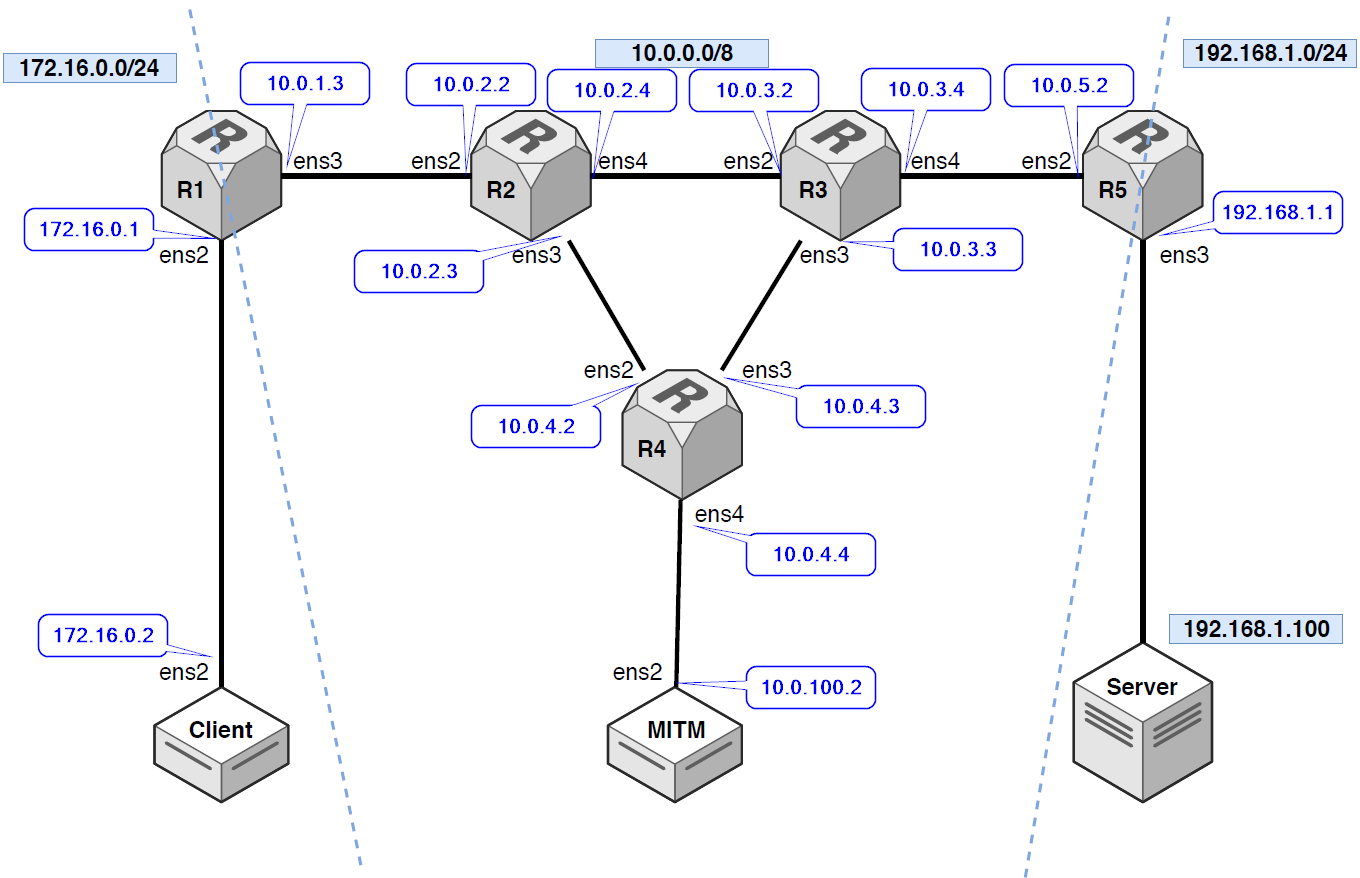
\includegraphics[width=0.90\textwidth]{images/netplan.png}
    \caption{Netplan}
    \label{fig:Netplan}
  \end{center}
\end{figure}

Die Adressen sind so definiert, dass jede Verbindung ein eigenes Subnet hat. Bird sucht seine Nachbarn anhand des Broadcasts.

Wir ändern den netplan mit \lstinline!sudo nano /etc/netplan/50-cloud-init.yaml!.


\lstinputlisting[language=bash,caption={/etc/netplan/50-cloud-init.yaml on R1}]{configs/R1/etc/netplan/50-cloud-init.yaml}

Mit \lstinline!netplan apply! übernehmen wir die neu definierten IP-Adressen.

\subsection{BIRD}
\label{subsec:BIRD}
\begin{shadedquotation}
  Now, your routers must run OSPF. ...
  \begin{itemize}
    \item OSPFv2 must run on the routers.
    \item Find a way to protect the CPU from too much OSPF processing.
    \item A restart of BIRD should not result in lost routes.
  \end{itemize}
\end{shadedquotation}

Wir definieren die Configuration von Bird indem wir ''/etc/bird/bird.conf'' anpassen.

Um die Auslastung von CPU und Netzwerk zu vermindern, haben wir uns an \cite{ReducingBGP} orientiert.

\lstinputlisting[language=bash,caption={/etc/bird/bird.conf on R1}]{configs/R1/etc/bird/bird.conf}

Zuerst definierten wir die ''router id'' nach Vorgabe.
\medskip
Unter ''protocol kernen'' definierten wird dass alle routes in die kernel routing table exportiert werden und dort persistent sind, dadurch funktioniert das Routing weiterhin wenn Bird beendet wird.

\medskip
Unter ''protocol static'' werden statische routes eingetragen. Nur R1 und R5 haben dort Einträge um ein routing nach Aussen / Innen des Routing-Netzwerkes zu ermöglichen.

\medskip
Unter ''protocol ospf'' definieren wird das Verhalten des OSPF. Wir setzten ''tick'' auf 5, dadurch werden Änderungen innerhalb von 5 Sekunden gesammelt, bevor diese ausgeführt werden. Dadurch wird das Netzwerk weniger geflutet und die CPU ausgelastet.

Wir definieren dass die ''area 0'' aus den Netzwerken ''10.0.0.0/8'', ''172.16.0/24'' und ''192.168.1.0/24'' besteht. Dadurch weiss OSPF, welche Adressen geroutet werden sollen.

Zusätzlich definieren wir, welche Interface von OSPF verwendet werden sollen. Dort definieren wir auch, in welchem Intervall zum Beispiel ein ''hello'' geschickt wird.
Um ebenfalls das fluten des Netzwerks zu minimieren, werden gewisse Werte höher gesetzt als der Standartwert.

Zum Schluss definieren wir, das alle restlichen Interfaces ''stub'' sind und daher zu ignorieren sind.

\medskip
Wir haben eine Vorlage aus dem Internet übernommen \cite{BIRD_EXAMPLE} und die einzelnen Einstellungen anhand von \cite{BIRD_DOC} überprüft und angepasst.

\subsection{IP Forwarding}
\label{subsec:IPForwarding}

''IP-Forwarding'' ist standartgemäs ausgeschaltet. Mit \lstinline!sysctl net.ipv4.ip_forward=1! aktivieren wird das weiterleiten der Packete erlaubt.

\par\medskip

\subsection{Script}
\label{subsec:Script}

Da wir keine Ahnung von ''Bird'' hatten, wurde das Anpassen und Testen der Configuration aufwendig, weshalb wir kurzer Hand ein Script erzeugten, welche die zuvor definierten Einstellungen anwendet:

\lstinputlisting[language=bash,caption={~/doConfig.sh}]{configs/doConfig.sh}

\section{Verifizierung}
\label{sec:Verifizierung}
\begin{shadedquotation}
  Verify your routing implementation. Explain which exact commands you used for each verification step and show how they provide prove that your setup works.
\end{shadedquotation}
Zuerst haben wir die IP-Vergabe überprüft und von jedem Router aus seine Nachbarn mit dem Befehl \lstinline!ping! angepingt. So haben wir als Beispiel von ''R3'' aus ''R2'', ''R4'' und ''R5'' angepingt.
Alle Pings waren erfolgreich.

\medskip

Anschliessend haben wir von ''R1'' jedes andere Gerät mit \lstinline!ping! angepingt und so erkennen können, dass die Routes funktionieren. Zusätzlich haben wir auch eine Routes genauer mit \lstinline!tcptraceroute! untersucht und konnten die Verbindung anhand des Netplans (\autoref{fig:Netplan}) nachverfolgen.  

\subsection{Route Failover}
\label{subsec:RouteFailover}
\begin{shadedquotation}
  Verify that your setup works. Prove that a route failover takes place in case ofa route outage. To do that, a well known tool can be used.
\end{shadedquotation}

Wir haben manuell gewisse Interfaces der Router mit \lstinline!ifconfig ens2 down! ausgeschaltet haben während ein anderer Routern \lstinline!ping! ausgeführt hat. Es dauerte zwar einige Sekunden (etwa 10 Sekunden) bis die Verbindung wieder stand, aber der Route Failover funktionierte.

\medskip

Wir haben von ''R1'' aus nach ''Server'' \lstinline!tcptraceroute!d und bei ''R3'' jeweils die Interface aus- und eingeschaltet.

\begin{figure}[H]
  \begin{center}
    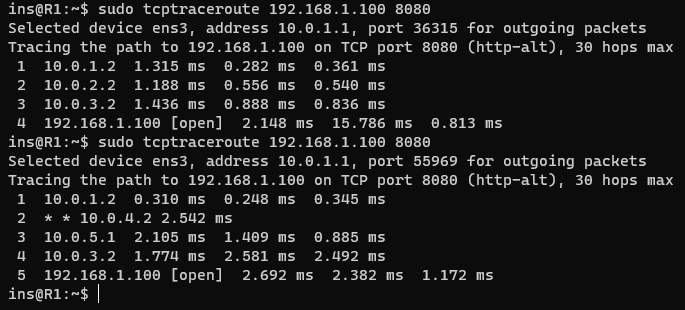
\includegraphics[width=0.90\textwidth]{images/tcptracert_R3-ens2-down.png}
    \caption{Tracert von R1 zu Server: R3-ens2 down}
    \label{fig:RouteFailoverDown}
  \end{center}
\end{figure}

\begin{figure}[H]
  \begin{center}
    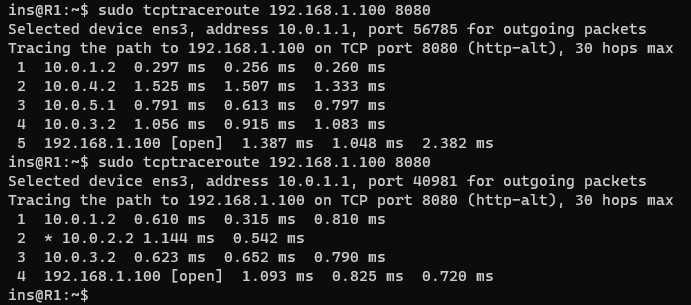
\includegraphics[width=0.90\textwidth]{images/tcptracert_R3-ens2-up.png}
    \caption{Tracert von R1 zu Server: R3-ens2 up again}
    \label{fig:RouteFailoverUp}
  \end{center}
\end{figure}


\subsection{Passive Interfaces}
\label{subsec:PassiveInterfaces}
\begin{shadedquotation}
  Show that no OSPF packets are sent into the client and server networks,too.\lstinline!tcpdump! and \lstinline!tshark! are good tools for that, sniff on the suspicious interfaces and filter for OSPFv2 packets. To be sure that your filter works, sniff on an interface where you expect OSPF-messages, too.
\end{shadedquotation}

Wir haben versucht, anhand von Wireshark mit ''Sshdump'' und ''Ciscodump'' auf den Interfaces zu lauschen, erhielten aber keine Pakete.
Wir versuchten ebenfalls mit \lstinline!tcpdump! die Pakete aufzufangen. Dies klappe zwar, aber das pcap-File wollte sich einfach nicht übertragen lassen. Wir sind anhand von \cite{TCPDUMP} vorgegangen.

\medskip

Mit TCPDump konnten wir die Pakete sehen und damit verifizieren, dass keine OSPF Pakete an das Client-, sowie Server-Netzwerk gesendet werden.

\begin{figure}[H]
	\begin{center}
		\includegraphics[width=0.90\textwidth]{"images/R1 OSPF Capture"}
		\caption{R1 ens3 Capture}
		\label{fig:R1-OSPF-Capture}
	\end{center}
\end{figure}

\begin{figure}[H]
	\begin{center}
		\includegraphics[width=0.90\textwidth]{"images/Client OSPF Capture"}
		\caption{Client ens2 Capture}
		\label{fig:client-OSPF-Capture}
	\end{center}
\end{figure}

\begin{figure}[H]
	\begin{center}
		\includegraphics[width=0.90\textwidth]{"images/R5 OSPF Capture"}
		\caption{R5 ens3 Capture}
		\label{fig:client-OSPF-Capture}
	\end{center}
\end{figure}


\subsection{Access Website}
\label{subsec:AccessWebsite}
\begin{shadedquotation}
  Finally, you must be able to access the webpage from the webserver. You can use \lstinline!curl! or \lstinline!wget! for that. The webserver listens on port 8080.
\end{shadedquotation}
Der Zugriff auf die Webseite ist möglich.
\begin{figure}[H]
	\begin{center}
		\includegraphics[width=0.90\textwidth]{"images/Verifikation Access Website"}
		\caption{Access Website}
		\label{fig:verifikation-access-website}
	\end{center}
\end{figure}

\section{Performanz}
\label{sec:Performanz}
\begin{shadedquotation}
  Provide the measurement before and after the appliance of the \lstinline!tc! commands.
  
  Provide the exact used \lstinline!tc! commands.
\end{shadedquotation}

\section{Firewall}
\label{sec:Firewall}
\begin{shadedquotation}
	The next step is to implement a firewall in your network. On Linux, netfilter was the kernel
	firewall for a long time. To configure netfilter, tools like iptables, ip6tables, arptables and so
	on were used. But for this task, you’ll have to use the more modern nftables and its nft utility
	to configure it.
	First, check all open ports of the webserver from your client with nmap. Your firewall solution
	must fulfill the following requirements:
	\begin{itemize}
		\item You must use nftables and its utility nft. Do not use iptables.
		\item The firewall must run on one of the routers.
		\item The website is only accessible from the clients network (172.16.0.0/24).
		\item Pings must not be answered.
		\item nmap must not show any open ports. Check if your firewall works by executing nmap again.
	\end{itemize}
\end{shadedquotation}

\begin{shadedquotation}
  We’re interested in the used \lstinline!nmap! command, where the firewall runs and why you’ve choosen that location. Print the ruleset of the firewall and attach it to your report.
\end{shadedquotation}

Das Router-Netzwerk ''10.0.0.0/8'' sollte unserer Meinung nach keine anderen Komponenten enthalten asl Router, daher würden wir die Firewall jeweils an den Ein- und Ausgängen zum Netzwerk platzieren. Das wäre auf ''R1'' und ''R5''.
\medskip
Nach der Definition, das nur eine Firewall definiert werden soll, gehen wir davon aus, dass das Netzwerk ''172.16.0.0/24'' das Internet (oder VPN-Netzwerk) ist. Demnach müssen wir unser Router- und DMZ-Netzwerk schützen, was die Position der Firewall möglich am Anfang nötigt macht. Die Firewall wird also auf ''R1'' etabliert.
\medskip

\section{Referenzblatt}
\label{sec:Referenzblatt}
\begin{shadedquotation}
  We also expect you to hand in a reference sheet for all the net-work commands used in this lab. Just list every command and its function. This reference must not be longer than one page.
\end{shadedquotation}

\par\medskip 

\begin{tabular}{ |p{4cm}|p{10cm}|}
  \hline
  \textbf{Befehl} & \textbf{Funktion} \\
  \hline
  \lstinline! sudo nano <Pfad> ! & Öffnen eines Files im Texteditor \\
  \hline
  \lstinline! sudo hostname <newHostName>! & Zum ändern des Hostnames \\
  \hline
  \lstinline! sudo passwd! & Ändert das Passwort des aktuellen Benutzers. \\
  \hline
  \lstinline! sudo birdc ! & Zum kommunizieren mit einem laufenden BIRD. Einzelne Befehle, die hier nicht aufgeführt sind, sind auf \cite{BIRD_COMMAND} zu finden. \\
  \hline
  \lstinline! sudo birdc show status ! & Anzeigen vom router status, BIRD version, Laufzeit und Zeitpunkt von der letzten Rekonfiguration. \\
  \hline
  \lstinline! sudo birdc show interfaces ! & Anzeigen der Liste von allen Interfaces. Zeigt für jedes Interface, Typ, Status, MTU und die zugewiesene Adresse an.\\
  \hline
  \lstinline! sudo birdc show ospf interface ! & Anzeigen von detailierten Informationen über die OSPF Interfaces. \\
  \hline
  \lstinline! birdc show ospf neighbors ! & Anzeigen der Liste mit allen OSPF Nachbaren deren Zustand. \\
  \hline
  \lstinline! birdc show ospf state ! & Anzeigen von detailierten Informationen über OSPF Bereiche basierend auf der link-state database. Es zeigt die Netzwerk Topolgie, stub Netzwerke, zusammengeführte Netzwerke und Router von anderen Areas und externen Routen. Ausserdem zeigt es erreichbare Netzwerk Knoten an. \\
  \hline
  \lstinline! ping -c <num> <ip> ! & sendet num mal einen Ping an  die ip \\
  \hline
  \lstinline! tcptraceroute <ip> ! & Zum Anzeigen vom Pfad im Netzwerk vom Host, auf dem die Traceroute ausgeführt wird, und der angegebenen IP, sowie dem Ort, an dem die Route, falls vorhanden, nicht abgeschlossen werden kann und allen Hops bis zum Ziel. \\
  \hline
  \lstinline! sysctl net.ipv4.ip_forward=1 ! & Mit dem Befehl wird das weiterleiten der Packete erlaubt. \\
  \hline
  \lstinline! sudo reboot ! & Neustarten des Geräts. \\ 
  \hline
  \lstinline! sudo ifconfig ens* down/up ! & stellt ens* network interface ab/ein\\
  \hline
  \lstinline! sudo tcpdump --interface <interface> ! & hört auf dem interface mit und zeigt alle pakete\\
  \hline
  \lstinline! curl <ip>:<port> ! & Aufruf von HTTP/HTTPS Files auf der IP und Port\\
\hline
\end{tabular}

\section{Anhänge}
\label{sec:Anhänge}

\subsection{Routing}
\label{subsec:Routing}
\begin{shadedquotation}
  \begin{itemize}
    \item Your delivered report must include the new usernames and pass-words of the hosts.
    \item Your delivery must contain the created netplan files and an ad-dress plan.
    \item Attach the BIRD config files to your cookbook and explain how you achieve the minimal requirements.
    \item Verify your routing implementation. Explain which exact commands you used for each verification step and show how they provide prove that your setup works.
  \end{itemize}
\end{shadedquotation}
Erarbeitung der BIRD-config ist im \ref{subsec:BIRD} erläutert.
Verifikation der Routing unter \ref{sec:Verifizierung}.

\subsection{Quellennachweis}
\label{subsec:Quellennachweis}

\begingroup
% Remove Titles eg "Literatur"
\renewcommand{\section}[2]{}%
% Reminder: Recreate "SmartFactory.bll" when "citavi/citavi.bib" gets changed => run BibTeX ([F11] in TexMaker)
\bibliography{Lab2_Quellen/quellen}
% Use the "IEEE standard" as style => "IEEEtran.bst"
\bibliographystyle{IEEEtran}
\endgroup  

\section{Nachwort}
\label{sec:Nachwort}

Kein Mitglied unserer Gruppe hat CN2 besucht. Alleine bis wir \ref{subsec:BIRD} zum laufen brachten haben wir gemeinsam mehr als 30 Stunden aufgewendet. 


\end{document}
